To introduce the \textbf{Fisher Information} (FI), we will start off with how it is defined and used in statistics.\\
Let's define a statistical model $f(x_i|\theta)$ that represents how a parameter $\theta$ is related to the outcomes $x_i$ of random variables $X_i$\cite{StatisticFisherInfoTutorial}. As an example of what this means, lets look at a Galton board. For readers that are not familiar with a what Galton boards are, there is an example photograph in \cref{fig:GaltonPicture}. 
\begin{figure}
	\centering
	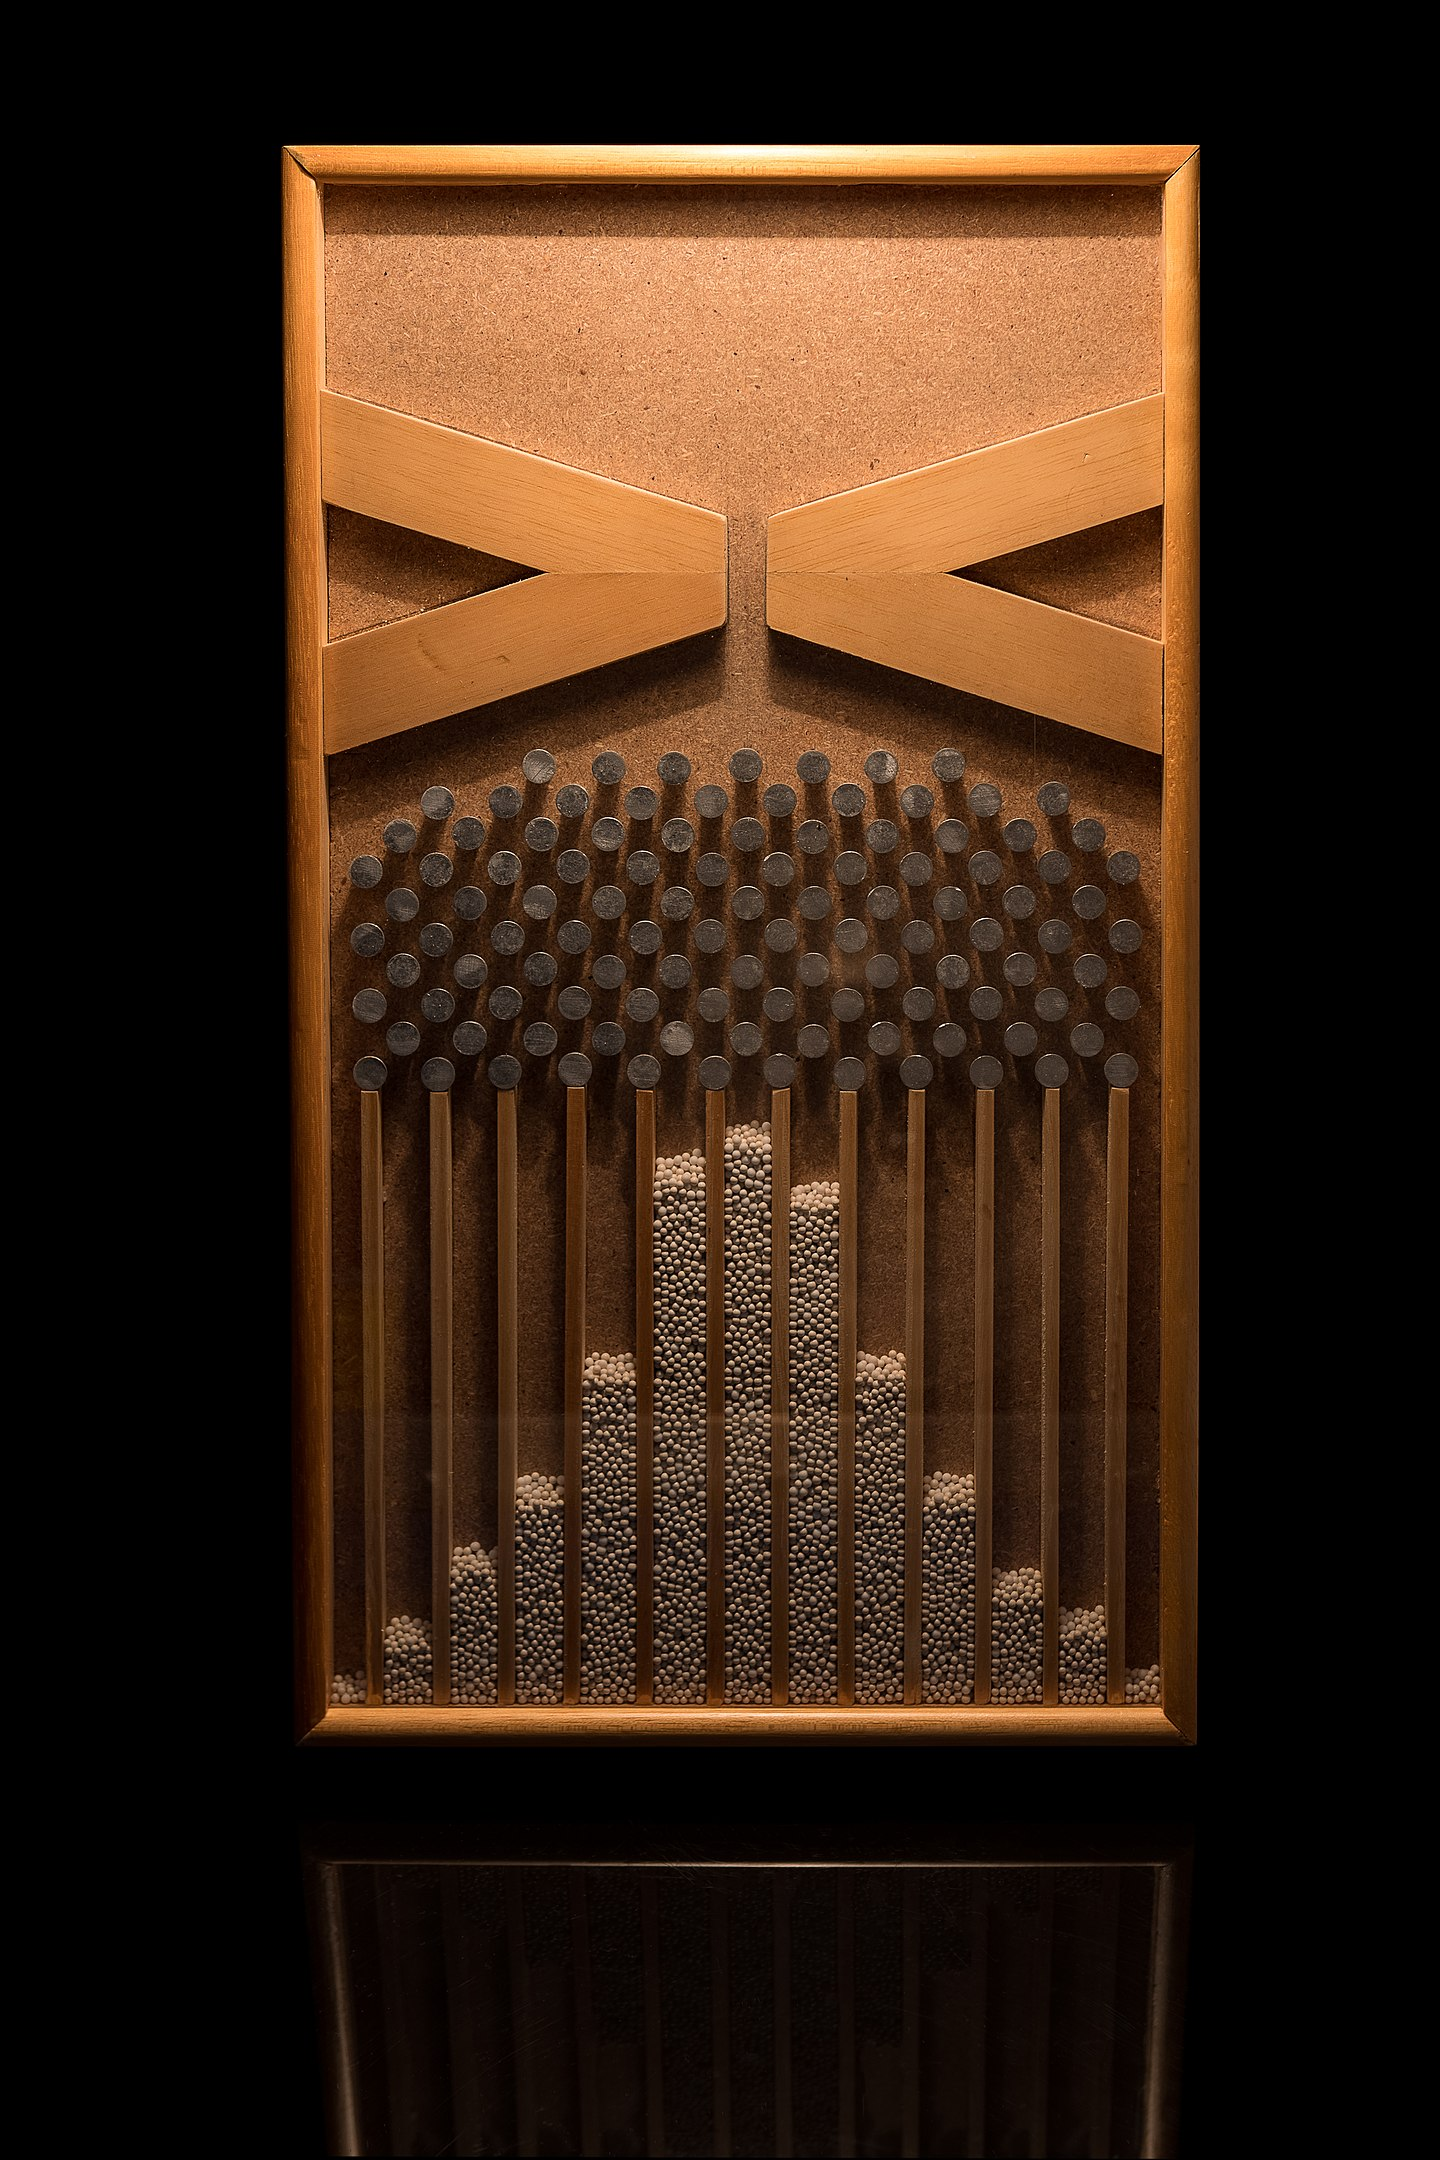
\includegraphics[width = 4cm]{text/FisherInformation/plots/GaltonBoard.jpg}
	\caption{This figure shows a picture of a Galton board. Taken from \cite{GaltonBoardPicture}.}
	\label{fig:GaltonPicture}
\end{figure}
It's a famous mechanical model that shows binomial distributions, which are approximations of the normal distribution. If we place many balls at the top of the board and let them fall to the bottom, the amount of balls that end up in each cell are distributed according to the binomial distribution. In this case, $x_i$ could assume the slot number which a ball can fall into. The $i$ could label multiple throws into the board. To introduce a parameter that influences the distribution of balls, let's say one can throw from different spots above the Galton board which we now control with the the value of $\theta$. For a known $\theta$, the resulting value of the statistical model represents the probability distribution $p_\theta(x_i)$ for the probability of the different $x_i$ outcomes. A visual representation of the probability distributions for different $\theta$ can be seen in \cref{fig:GaltonDistributions}.
\begin{figure}
	\centering
	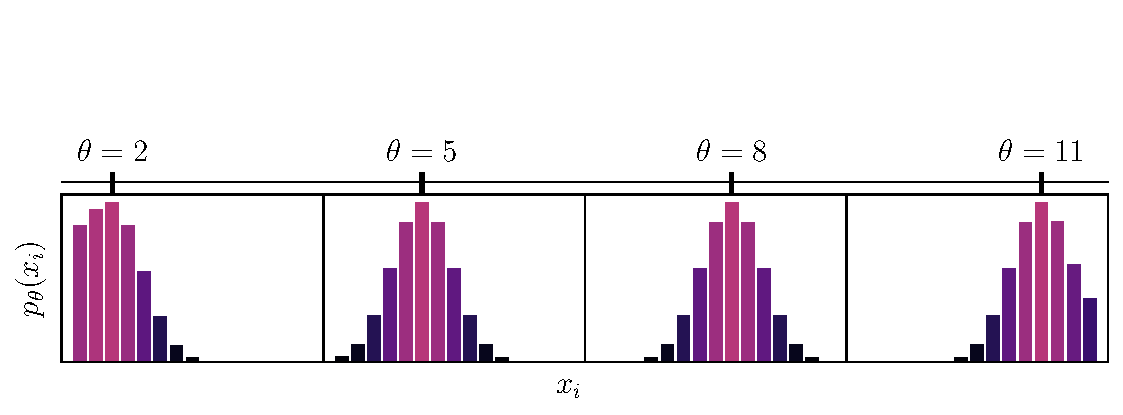
\includegraphics[width = \textwidth, clip, trim= 0cm 0cm 0cm 2.3cm]{text/FisherInformation/plots/GaltonDistributionsPlot.pdf}
	\caption{This figure shows the probability distributions for a Galton boards with different drop in position. The slots where the ball can end up are labeled by the value of $x_i$.}
	\label{fig:GaltonDistributions}
\end{figure}\\
In general, the statistical models might be more complex, with $\theta$ containing multiple parameters, $x$ being an element of a mathematical space other than $\mathbb{R}$ and the index $i$ denoting various different experiments that all depend on the same parameter but have different possible outcomes and probability distributions.\\
What's of interest for the FI are cases where the parameters are not known before conducting the experiment, and have to be approximated by the different outcomes $x_i$.\\
Before we introduce the FI, let's look at an example from \cite{StatisticFisherInfoTutorial}. Let's consider a biased coin where we denote the probability for heads ($x_i = 1$) with $\theta$. The probability for tails ($x_i = 0$) is then $1-\theta$. We will now take a look at the outcome of $n$ throws represented by the variable $X^n$. For example one observed result for $X^5$ could be $x = (1,1,0,1,0)$. Lets consider another variable $Y$ whose observation is the sum of the total head throws $y = \sum x$. In our example case of $x = (1,1,0,1,0)$ this would result in a value of $y = 3$. The probability for this variable $y$ is distributed according to the binomial distribution, which means $f(y|\theta) = \binom{n}{y}\theta^y \theta^{n-y}$. Here the binomial coefficient $\binom{n}{y}$ represents the different combinations that result in the same $y$ value. This is needed because there are $2^n$ different possibilities for $x$ while there are only $n$ different possibilities for $y$.\\
If we now fix the outcome of $y$ and look at the conditional probability for the different $x$ that could have resulted in that $y$ value, we get $p(x|y,\theta) = 1/ \binom{n}{y}$. Although the probability of $y$ and $x$ both depend on $\theta$, the probability for $x$ when $y$ is fixed doesn't. This means that $y$ is fully descriptive of or "sufficient for" the parameter $\theta$. Measuring $y$ results in the same amount of information about the parameter $\theta$ as measuring the whole observation $x$. To quantify how much information a certain function of outputs $t(x)$ contains about the parameters $\theta$ Fisher introduced the Fisher information.\\
